\subsection{Степенные ряды}

\begin{definition}
    Пусть $a_n\in \C$, $z_0\in \C$. $\sum\limits_{n=0}^\infty a_n\underbrace{(z-z_0)^n}_{:=w^n}$ – \textit{степенной ряд}.

    $\sum\limits_{n=0}^\infty a_nw^n$, $w = z-z_0$.
\end{definition}

\begin{theorem}
    Если ряд $\sum\limits_{n=0}^\infty a_nz^n$ сходится при $z=z_0$, то ряд сходится (и даже абсолютно сходится) при $|z|<|z_0|$. Если ряд расходится при $z=z_0$, то он расходится при $|z|>|z_0|$.
\end{theorem}

\begin{proof}
    $\sum\limits_{n=0}^\infty a_nz^n$ – сходится $\Rightarrow a_nz_0^n\underset{n\rightarrow \infty}{\rightarrow} 0$ (необходимое условие) $\Rightarrow a_nz_0^n$ – ограниченная последовательность: $|a_nz^n_0|< M\ \forall n\Rightarrow |a_nz^n|=|a_nz_0^n|\cdot |\frac{z}{z_0}|^n\leq M |\frac{z}{z_0}|^n $ и $\sum\limits_{n=0}^\infty M|\frac{z}{z_0}|^n$ сходится ($\frac{z}{z_0}<1$ – геометрическая прогрессия) $\Rightarrow\sum a_nz^n$ абсолютно сходится по признаку сравнения.

    Второе утверждение – отрицание первого.
\end{proof}

\begin{definition}
    \textit{Радиус сходимости степенного ряда} $\sum\limits_{n=0}^\infty a_nz^n$ – такое $R\in [0, +\infty)$, что ряд сходится при $|z|<R$ и расходится при $|z|>R$.
    
    \textit{Круг сходимости степенного ряда} $\sum\limits_{n=0}^\infty a_nz^n$ – круг  $|z|<R$.

    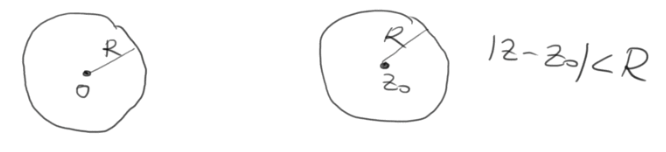
\includegraphics[width=0.5\linewidth]{images/10-05-1.png}
\end{definition}

\begin{theorem}
    \textbf{Формула Коши-Адамара}

    Всякий степенной ряд имеет радиус сходимости и он равен $R:=\frac{1}{\overline{\lim}\sqrt[n]{|a_n|}}$.
\end{theorem}

\begin{proof}
    Рассмотрим ряд $\sum\limits_{n=0}^\infty a_nz^n$. Применим признак Коши для $\sum\limits_{n=0}^\infty |a_nz^n|$:
    
    $q:=\overline{\lim}\sqrt[n]{|a_nz^n|}=\overline{\lim}\sqrt[n]{|a_n|}\cdot|z|$.

    Если $q<1$, то ряд сходится. $   \quad q<1\Leftrightarrow \overline{\lim} \sqrt[n]{|a_n|}\cdot |z|<1\Leftrightarrow |z|<\frac{1}{\overline{\lim} \sqrt[n]{|a_n|}}=R$.

    Если $q>1$, то члены ряда не стремятся к 0. $\quad q>1\Leftrightarrow |z|>R\Rightarrow \sum a_nz^n$ расходится.
\end{proof}

\begin{remark}
    Внутри круга сходимости ряд абсолютно сходится.
\end{remark}

\begin{example}~
    \begin{enumerate}
        \item $\sum\limits_{n=0}^\infty \frac{z^n}{n!}\quad R:=\frac{1}{\overline{\lim}\sqrt[n]{\frac{1}{n!}}}=\lim \sqrt[n]{n!}=+\infty$

        $n!\sim n^ne^{-n}\sqrt{2\pi n}$

        $\sqrt[n]{n!}\sim\frac{n}{e}$
        \item $\sum\limits_{n=0}^\infty n!z^n\quad R=0$

        \item $\sum\limits_{n=1}^\infty \frac{z^n}{n^2}$ – сходится при $|z|\leq 1$, при $|z|>1$ расходится.

        \item $\sum\limits_{n=0}^\infty z^n\quad R=1$ – при $|z|\geq 1$ ряд расходится, так как члены $\not\rightarrow 0$.
    \end{enumerate}
\end{example}

\begin{theorem}
    Пусть $R$ – радус сходимости ряда $\sum\limits_{n=0}^\infty a_nz^n$ и $0<r<R$. Тогда ряд равномерно сходится в круге $|z|\leq r$.

    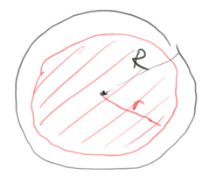
\includegraphics[width=0.2\linewidth]{images/10-05-2.png}
\end{theorem}

\begin{proof}
    Ряд $\sum\limits_{n=0}^\infty a_nz^n$ абсолютно сходится (из определения радиуса сходимости) $\Rightarrow\sum\limits_{n=0}^\infty |a_n|r^n$ сходится.

    $|a_nz^n|\leq |a_n|r^n$ при $|z|\leq r\overset{\text{пр. Вейерш.}}{\Rightarrow}$ $\sum\limits_{n=0}^\infty a_nz^n$ равномерно сходится при $|z|\leq r$.
\end{proof}

\begin{corollary}
    Сумма степенного ряда в круг сходимости – непрерывная функция.
\end{corollary}

\begin{proof}
    Проверяем непрерывность в точке $z_0$, $|z_0|<R$. Возьмем $|z_0|<r<R$. Знаем, что в круге $|z|\leq r$ есть равномерная сходимость $\Rightarrow$ там сумма ряда непрерывна $\Rightarrow$ есть непрерывность в точке $z_0$.

    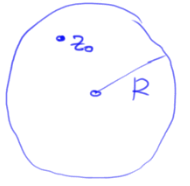
\includegraphics[width=0.2\linewidth]{images/10-05-3.png}
\end{proof}

\begin{theorem}
    \textbf{Теорема Абеля}

    Пусть $R$ – радиус сходимости ряда $\sum\limits_{n=0}^\infty a_nz^n$ и ряд сходится при $z=R$. Тогда на $[0, R]$ ряд сходится равномерно.
\end{theorem}
\begin{proof}
    $\sum\limits_{n=0}^\infty a_nx^n=\sum\limits_{n=0}^\infty a_nR^n\cdot (\frac{x}{R})^n$, $x\in [0, R]$

    $\sum\limits_{n=0}^\infty a_nR^n$ равномерно сходится (так как не зависит от $x$), $(\frac{x}{R})^n$ монотонно убывает, $0\leq (\frac{x}{R})^n\leq 1$
    
    $\overset{\text{пр. Абеля}}{\Rightarrow}$ ряд равномерно сходится.
\end{proof}

\begin{corollary}
    В условиях теоремы сумма $f(x):=\sum\limits_{n=0}^\infty a_nx^n: [0, R]\rightarrow \C$ – непрерывна на $[0, R]$ (слагаемые непрерывны + ряд равномерно сходится).

    В частности, $\lim\limits_{x\rightarrow R_-}\sum\limits_{n=0}^\infty a_nx^n=\sum\limits_{n=0}^\infty a_nR^n$ (непрерывность в точке $R$).
\end{corollary}

\begin{lemma}
    Пусть $x_n, y_n\in \R$, $\lim x_n\in (0, +\infty)$. Тогда $\overline{\lim }\ x_n y_n=\lim x_n\cdot \overline{\lim }\ y_n$.
\end{lemma}

\begin{proof}
    Пусть $A:=\lim x_n$, $B:=\overline{\lim}\ y_n$ и $C:=\overline{\lim}\ x_ny_n$. 
    
    $C$ – верхний предел, тогда $\exists x_{n_k}y_{n_k}\rightarrow C\Rightarrow x_{n_k}\rightarrow A\Rightarrow y_{n_k}\rightarrow\frac{C}{A}\rightarrow \frac{C}{A}\leq B$, так как $B$ – наибольший из всех частичных пределов.

    Возьмем $n_j: y_{n_j}\rightarrow B\Rightarrow x_{n_j}y_{n_j}\rightarrow A\cdot B\Rightarrow AB\leq C$

    Вывод: $AB=C$.
\end{proof}

\begin{corollary}
    Радиусы сходимости рядов $\sum\limits_{n=0}^\infty a_nz^n$,  $\sum\limits_{n=0}^\infty na_nz^{n-1}$ и $\sum\limits_{n=0}^\infty a_n\frac{z^{n+1}}{n+1}$ совпадают.
\end{corollary}

\begin{proof}
    Радиусы сходимости $\sum\limits_{n=0}^\infty na_{n}z^{n-1}$ и $\sum\limits_{n=0}^\infty na_{n}z^n$ совпадают (радиус не меняется от умножения на какое-то ненулевое число $z$).

    Радиусы сходимости $\sum\limits_{n=0}^\infty a_n\frac{z^{n+1}}{n+1}$ и $\sum\limits_{n=0}^\infty a_{n}\frac{z^n}{n+1}$ совпадают (опять же отличаются на $z$).

    То есть надо доказать, что  $\sum\limits_{n=0}^\infty a_{n}z^{n}$, $\sum\limits_{n=0}^\infty na_{n}z^n$ и $\sum\limits_{n=0}^\infty\frac{a_n}{n+1}z^n$ имеют одинаковые радиусы сходимости, то есть (пользуюсь формулой Коши-Адамара), что $\overline{\lim}\sqrt[n]{|a_n|}=\overline{\lim}\sqrt[n]{n|a_n|}=\overline{\lim}\sqrt[n]{\frac{|a_n|}{n+1}}$.

    А это верно из леммы + $\lim \sqrt[n]{n}=\lim \sqrt[n]{\frac{1}{n+1}}=1$.
\end{proof}

\begin{remark}
    Второй ряд получен из первого почленным дифференцированием первого, а третий – почленным интегрированием.
\end{remark}

\begin{theorem}
    \textbf{Почленное интегрирование степенного ряда.}

    Пусть $R$ – радиус сходимости, $f(x)=\sum\limits_{n=0}^\infty a_n(x-x_0)^n$. Тогда при $|x-x_0|<R$ $\int\limits_{x_0}^xf(t)dt=\sum\limits_{n=0}^\infty a_n\frac{(x-x_0)^{n+1}}{n+1}$ и этот ряд имеет тот же радиус сходимости.

    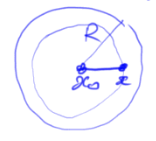
\includegraphics[width=0.2\linewidth]{images/10-05-4.png}
\end{theorem}

\begin{proof}
    На $[x_0, x]$ ряд равномерно сходится (так как отрезок целиком лежит в круге сходимости) $\Rightarrow$ можно интегрировать почленно.
\end{proof}

\begin{definition}
    Пусть $f: E\rightarrow \C$,  $E\subset \C$, $z_0$ – внутренная точка $E$. Если существует такое $k\in \C$, что $f(z)=f(z_0)+k(z-z_0)+o(z-z_0)$ при $z\rightarrow z_0$, то $f$ – \textit{комплексно-дифференцируема в точке} $z_0$.
\end{definition}

\begin{remark}~
    \begin{enumerate}
        \item $k=\lim\limits_{z\rightarrow z_0}\frac{f(z)-f(z_0)}{z-z_0}$ – \textit{производная $f$ в точке $z_0$}.
        \item Существование производной равносильно дифференцируемости.
    \end{enumerate}
\end{remark}

\begin{theorem}
    Пусть $R$ – радиус сходимости ряда $\sum\limits_{n=0}^\infty a_n(z-z_0)^n=:f(z)$. Тогда $f$ бесконечно дифференцируема в круге сходимости и $f^{(m)}(z)=\sum\limits_{n=0}^\infty n(n-1)...(n-m+1)a_n(z-z_0)^{n-m}$.
\end{theorem}

\begin{proof}
    Пусть $m=1$ (дальше индукция). 
    
    Возьмем $0<r<R$ и $|z|<r$, $|w|<r$.

    $\frac{f(w)-f(z)}{w-z}=\frac{1}{w-z}(\sum\limits_{n=1}^\infty a_nw^n - \sum\limits_{n=1}^\infty a_nz^n)=\sum\limits_{n=1}^\infty a_n\cdot \frac{w^n-z^n}{w-z}=\sum\limits_{n=1}^\infty a_n(w^{n-1}+w^{n-2}z+...+z^{n-1})$

    $\lim\limits_{w\rightarrow z}\frac{f(w)-f(z)}{w-z}=\lim\limits_{w\rightarrow z}\sum\limits_{n=1}^\infty a_n(w^{n-1}+w^{n-2}z+...+z^{n-1})\overset{?}{=}\sum\limits_{n=1}^\infty\lim\limits_{w\rightarrow z}a_n(w^{n-1}+w^{n-2}z+...+z^{n-1})=\sum\limits_{n=1}^\infty a_nnz^{n-1}$

    Про ?: $|a_n(w^{n-1}+w^{n-2}z+...+z^{n-1})|\leq |a_n|\cdot nr^{n-1}$, $\sum\limits_{n=0}^\infty n|a_n|r^{n-1}\overset{\text{пр. Вейерш.}}{\Rightarrow}$ нужный ряд равномерно сходится, то есть можно переставлять $\lim$ и $\sum$ местами.
\end{proof}

\begin{theorem}
    \textbf{Единственность разложения в степенной ряд.}

    Пусть $f(z)=\sum\limits_{n=0}^\infty a_n(z-z_0)^n$ при $|z-z_0|<R$ – радиус сходимости. Тогда $a_n=\frac{f^{(n)}(z_0)}{n!}$.
\end{theorem}

\begin{proof}
    Выведем формулу для коэффициентов:

    $f^{(m)}(z)=\sum\limits_{n=0}^\infty n(n-1)...(n-m+1)a_n(z-z_0)^{n-m}$. Подставим $z=z_0\Rightarrow f^{(m)}(z_0)=m\cdot(m-1)\cdot...\cdot1\cdot a_n=m!\cdot a_m$.
\end{proof}

\begin{definition}
    Пусть $f$ бесконечно дифференцируема в точке $z_0$. 
    
    Тогда ряд $f(z)=\sum\limits_{n=0}^\infty\frac{f^{(n)}(z_0)}{n!}
    (z-z_0)^n$ – \textit{ее ряд Тейлора в точке $z_0$}.
\end{definition}

\begin{definition}
    $f$ – \textit{аналитическая в точке} $z_0$, если в окрестности точки $z_0$ 
    
    $f(z)=\sum\limits_{n=0}^\infty\frac{f^{(n)}(z_0)}{n!}(z-z_0)^n$. 
\end{definition}

\begin{remark}
    $f$ – бесконечно дифференцируема $\not\Rightarrow$ аналитичность.
\end{remark}

\begin{example}
    $f: \R\rightarrow \R$, $f(x)=\left\{\begin{array}{ll}
         0, \quad x=0 \\ e^{-\frac{1}{x^2}},\quad x\neq 0
    \end{array}\right.$

    Проверим, что $f^{(n)}(x)=\left\{\begin{array}{ll}
         0, \quad x=0 \\ \frac{p_n(x)}{x^{3n}}\cdot e^{-\frac{1}{x^2}},\quad x\neq 0
    \end{array}\right.$

    Индукция. Переход $n\rightarrow n+1$, $x\neq 0$:

    $(f^{(n)}(x))'=(p_n(x)x^{-3n}e^{-\frac{1}{x^2}})'=p_n'(x)x^{-3n}e^{-\frac{1}{x^2}} +p_n(x)(-3n)x^{-3n} e^{-\frac{1}{x^2}} + p_n(x) x^{-3n} 3\cdot x^{-3}e^{-\frac{1}{x^2}}$

    $x=0$:

    $f^{(n+1)}(0)=\lim\limits_{x\rightarrow 0}\frac{f^{(n)}(x)-f^{(n)}(0)}{x-0}=\lim\limits_{x\rightarrow 0} \frac{f^{(n)}(x)}{x} =\lim\limits_{x\rightarrow 0} \frac{p_n(x)}{x^{3n+1}}\cdot e^{-\frac{1}{x^2}} = \lim\limits_{y\rightarrow \infty}p_n(\frac{1}{y})y^{3n+1}e^{-y^2}=0$

    Есть бесконечная дифференцируемость. 
    
    Формула Тейлора при $x_0=0$: $\sum\limits_{n=0}^\infty\frac{f^{(n)}(0)}{n!}x^n=0$, но $f(x)\neq 0$ при $x\neq 0$.
\end{example}

\subsection*{Разложение элементарных функций в ряд Тейлора}
\begin{enumerate}
    \item $e^x=\sum\limits_{n=0}^\infty\frac{x^n}{n!}$
    \item $\cos x=\sum\limits_{n=0}^\infty(-1)^n\frac{x^{2n}}{(2n)!}$
    \item $\sin x=\sum\limits_{n=0}^\infty(-1)^n\frac{x^{2n+1}}{(2n+1)!}$
\end{enumerate}

Ряд сходятся $\forall x\in \R\Rightarrow$ сходятся $\forall x\in \C$.

\begin{definition}
    Пусть $z\in \C$, тогда: 
    
    \begin{enumerate}
        \item[1)] $e^z=\sum\limits_{n=0}^\infty\frac{z^n}{n!}$
        \item[2)] $\cos z=\sum\limits_{n=0}^\infty(-1)^n\frac{z^{2n}}{(2n)!}$
        \item[3)] $\sin z=\sum\limits_{n=0}^\infty(-1)^n\frac{z^{2n+1}}{(2n+1)!}$
    \end{enumerate}
\end{definition}

\textbf{Формула Эйлера:}

$e^{iz}=\cos z+i\sin z$

\begin{exercise}
    Доказать, что:
\begin{enumerate}
    \item $\sin^2z+\cos^2z=1$
    \item $\sin z=\frac{e^{iz}-e^{-iz}}{2}$
    \item $\cos z=\frac{e^{iz}+e^{-iz}}{2}$
    \item $e^{z+w}=e^z\cdot e^w$
\end{enumerate}
\end{exercise}



\begin{enumerate}
    \item[4)] $\ln(1+x)=\sum\limits_{n=0}^\infty (-1)^{n-1}\frac{x^n}{n}$ при $x\in (-1, 1)$.
\end{enumerate}

\begin{proof} 
    $\ln (1+x) =\int\limits_0^x\frac{dt}{1+t}\overset{\text{геом. прогр.}}{=}\int\limits_0^x \sum\limits_{n=0}^\infty(-1)^nt^ndt = \sum\limits_{n=0}^\infty(-1)^n \int\limits_0^x t^ndt = \sum\limits_{n=0}^\infty (-1)^n\frac{x^{n+1}}{n+1}$
\end{proof}

\begin{enumerate}
    \item[5)] $\arctan x=\sum\limits_{n=0}^\infty (-1)^{n-1}\frac{x^{2n+1}}{2n+1}$ при $x\in (-1, 1)$.
\end{enumerate}

\begin{proof}
    $\arctan x =\int\limits_0^x\frac{dt}{1+t^2}\overset{\text{геом. прогр.}}{=}\int\limits_0^x \sum\limits_{n=0}^\infty(-1)^nt^{2n}dt = \sum\limits_{n=0}^\infty(-1)^n \int\limits_0^x t^{2n}dt = \sum\limits_{n=0}^\infty (-1)^n\frac{x^{2n+1}}{2n+1}$
\end{proof}

\begin{enumerate}
    \item[6)] $(1+x)^p=1+px+\frac{p(p-1)}{2}x^2+...+\frac{p(p-1)...(p-n+1)}{n!}x^n+...$ при $x\in (-1, 1)$.
\end{enumerate}

\begin{proof}
    Пусть $(1+x)^p=T_n(x)+R_n(x)$. Надо доказать, что $T_n(x)\underset{n\rightarrow +\infty}{\rightarrow} (1+x)^p$, то есть $R_n(x)\underset{n\rightarrow +\infty}{\rightarrow} 0$.

    Воспользуемся интегральной формулой для остатка: $R_n(x)=\frac{1}{n!}\int\limits_0^x (x-t)^n \underbrace{(1+t)^{p-n-1}p(p-1)...(p-n)}_{=f^{(n+1)}(t)}dt$

    Посмотрим на отношение: $|\frac{R_{n+1}(x)}{R_n(x)}|=\bigg|\frac{\frac{1}{(n+1)!}\int\limits_0^x (x-t)^{n+1} (1+t)^{p-n-2}p(p-1)...(p-n-1)dt}{\frac{1}{(n)!}\int\limits_0^x (x-t)^{n} (1+t)^{p-n-1}p(p-1)...(p-n)dt}\bigg|=\frac{|p-n-1|}{n+1}\cdot \frac{|\int\limits_0^x (x-t)^{n+1}(1+t)^{p-n-2}dt|}{|\int\limits_0^x (x-t)^{n}(1+t)^{p-n-1}dt|}$

    $=\frac{|p-n-1|}{n+1}\cdot \frac{\int\limits_0^x |x-t|^{n+1}(1+t)^{p-n-2}dt}{\int\limits_0^x |x-t|^{n}(1+t)^{p-n-1}dt}=\frac{|p-n-1|}{n+1}\cdot\frac{\int\limits_0^x |x-t|^{n}(1+t)^{p-n-1}\cdot \frac{|x-t|}{1+t}dt}{\int\limits_0^x |x-t|^{n}(1+t)^{p-n-1}dt}\leq \frac{|p-n-1|}{n+1} |x|\underset{n\rightarrow +\infty}{\rightarrow} |x|<1\Rightarrow$ члены последовательности стремятся к 0.

    $\frac{|x-t|}{1+t}\leq |x|$

    Если $x<0$: $(t-x)\leq (-x)(1+ t)=-x-tx\Leftrightarrow t\leq -tx \Leftrightarrow -1\leq x$
\end{proof}

\begin{example}
    Частный случай: $p=-\frac{1}{2}\quad \frac{1}{\sqrt{1+x}}=\sum\limits_{n=0}^\infty (-1)^n\frac{(2n-1)!!}{(2n)!!}x^n=\sum\limits_{n=0}^\infty(-1)^n\frac{\binom{2n}{n}}{4^n}x^n$
\end{example}

\begin{enumerate}
    \item[7)] $\arcsin x=\sum\limits_{n=0}^\infty \frac{\binom{2n}{n}}{4^n}\cdot \frac{x^{2n+1}}{2n+1}$
\end{enumerate}

\begin{proof}
    $(\arcsin x)'=\frac{1}{\sqrt{1-x^2}}$
\end{proof}